\documentclass{article}

\title{	
	\normalfont\normalsize 
	\rule{\linewidth}{0.5pt}\\ % Thin top horizontal rule
	\vspace{14pt} % Whitespace
	{\LARGE MATH428 Assignment 1 \\ % The assignment title
    \large \textit{} \\}
	\vspace{6pt} % Whitespace
	\rule{\linewidth}{1pt}\\ % Thick bottom horizontal rule
}

\author{Elliott Hughes}
\date{\normalsize\today}
\usepackage{tikz}
\usepackage{tikz-3dplot}
\usetikzlibrary{arrows,automata}
\usetikzlibrary{positioning}
\usetikzlibrary{arrows.meta,positioning}
\usetikzlibrary{calc}
\usetikzlibrary{shapes.geometric}
\tdplotsetmaincoords{80}{45}

\tikzset{surface/.style={draw=black, left color=red,right color=red,middle
color=red, fill opacity=1},surface/.default=white}

%% macros to draw back and front of cones
%% optional first argument is styling; others are z, radius, side offset (in degrees)
\newcommand{\coneback}[4][]{
  %% start at the correct point on the circle, draw the arc, then draw to the origin of the diagram, then close the path
  \draw[canvas is xy plane at z=#2, #1] (\tdplotmainphi-#4:#3) 
  arc(\tdplotmainphi-#4:\tdplotmainphi+180+#4:#3) -- (O) --cycle;
  }
\newcommand{\conefront}[4][]{
  \draw[canvas is xy plane at z=#2, #1] (\tdplotmainphi-#4:#3) arc
  (\tdplotmainphi-#4:\tdplotmainphi-180+#4:#3) -- (O) --cycle;
  }

\usepackage{mdframed}
\usepackage{amsmath}
\usepackage{amssymb}
\usepackage{graphicx}
\graphicspath{ {./Images/} }
\usepackage{commath}
\usepackage{textcomp}
\usepackage{gensymb}
\usepackage{float}
\usepackage{hyperref}
\usepackage[margin=1in]{geometry}
\usepackage{caption}
\usepackage{subcaption}
\usepackage{sectsty}
\usepackage{titlesec}
\usepackage{rotating}
\usepackage{pgfplots}

\begin{document}

\maketitle

\section*{Q1}
\subsection*{(a)}
Suppose $C$ is an open cover of $X'$ and let $O_{x'}$ be an element of this cover including 
$x'$. Since this set includes $x'$ it cannot be an element of $\tau$ so it must be of the form 
$O_{x'} = \{X'\backslash M: M \subset X \text{is compact}\}$ . Consider the set of sets 
containing $M$ formed 
by restricting each set in $C$ to $X$ (we will denote this restricted cover $C^M$). Each set in 
$C^M$ is an open set, as it is either an element of $\tau$ or of the form $X\backslash C$ (where 
$C$ is a compact set). Sets in $\tau$ are trivially open, while compact sets $X$ are compact sets in a Hausdorff space
and thus closed (so they have open complements). Thus $C^M$ is a cover of $M$ and 
$M$ is a compact set so it follows that there exists a finite subcover of $M$ $F^M$. Finally 
$F^M \cup O_{x'}$ is a cover of the whole space and is finite, so $(X',\tau')$ is compact.

\subsection*{(b)}
Under the Euclidean topology, $\mathbb{R}^2$ is homeomorphic to $S^2\backslash \{p\}$ 
under the topology induced by restricting the Euclidean topology to $S^2\backslash \{p\}$. 
Therefore we can define the function $f:\mathbb{R}^2\cup \{x'\} \rightarrow S^2$ by 

\begin{equation*}
    f = 
    \begin{cases}
        g(x) & x \in \mathbb{R}^2 \\
        p & x = x'
    \end{cases}
\end{equation*}

where $g(x)$ is a homeomorphism from $\mathbb{R}^2$ to $S^2\backslash \{p\}$. It remains to show that 
this is a homeomorphism. If one considers an open set $O_x \subseteq S^2\backslash \{p\}$ then 
clearly the preimage of this set is also an open set. Considering an open set $O_{p}$ containing $p$ 
one can write this set as $O \cup p$ where $O = O_{p} \backslash \{p\}$. Furthermore since 
$S^2$ is Hausdorff, $O_{p}$ is Hausdorff and so for all $x \in O$ there exists an neighborhood $N$  
of $x$ in the induced subspace topology of $O_p$ such that $N$ does not contain $x'$ and thus $N \subseteq O$. Thus $O$ is open and so the preimage of $O_{p}$ is the 
union of an open set in $\mathbb{R}^2$ and $x'$. Since $\mathbb{R}^2$ is a closed set under the 
Euclidean topology, $\{x'\}$ is an open set and so $O_p$ is the union of two open sets and thus 
open. Thus $f$ is continuous. Furthermore, it is by construction a bijection and 
thus these spaces are homeomorphic.

\section*{Q2}
Clearly this annulus is a closed and bounded subset of 
$\mathbb{R}^2$ and must thus be compact. Furthermore $S^2$ is Hausdorff, so if there exists a 
continuous map from the annulus to $S^2$ then the induced identification space is homeomorphic to 
$S^2$. Without loss of generality we will set $S^2$ to be the unit circle centred at the origin. 
For convenience we will write the annulus in polar coordinates $(\theta, r)$ and the sphere in (unsurprisingly) 
spherical coordinates $(\theta, \psi, r)$

\begin{equation}
    f(\theta, r) = \left(\theta, \frac{\pi (r-1)}{3}, 1\right)
\end{equation}

this function is obviously continuous and onto, so the identification space $A/\sim_f$ is 
homeomorphic to the sphere (by theorem 5.10). Furthermore, $A/\sim_f$ identifies 
all points at the outer boundary of the annulus to a single point (which is mapped to the 
South pole of the sphere under $f$) and all points at the inner 
boundary to a single point mapped to the North Pole under $f$. For convenience we will denote 
these points $n$ and $s$, leading to the following diagram (\autoref{fig:Q2_AS2}):

\begin{figure}[H]
    \centering
    \begin{tikzpicture}

        % Define radius and center points
        \def\r{3}
        \node (sphere_orig) at (5,0) {};
        \node (annulus_orig) at (-5,0) {};
        
        % Sphere
        \draw (sphere_orig) circle (\r);
        \draw[dashed] (sphere_orig) ellipse (\r{} and \r/3);
        \node[circle, draw=red, fill = red, minimum size = 2mm, inner sep = 0.4, label = above:$n$] (n_pole) at ($ (sphere_orig) +(0,3)$) {};
        \node[circle, draw=blue, fill = blue, minimum size = 2mm, inner sep = 0.4, label = below:$s$] (s_pole)  at ($ (sphere_orig) +(0,-3)$) {};

        % draw the matching annulus
        \draw[blue, thick] (annulus_orig) circle (\r);
        \draw[red, thick] (annulus_orig) circle (1);

        % labels
        \node (sphere_label) at ($(sphere_orig) + (0,-4.5)$) {\large$S^2$};
        \node (annulus_label) at ($(annulus_orig) + (0,-4.5)$) {\large$A/\sim_f$};

      
      \end{tikzpicture}
      \caption{The identification space induced by $f$ and the sphere. Points in blue (red) on $A/ \sim_f$ are mapped 
      to the blue (red) point on $S^2$.}
      \label{fig:Q2_AS2}
\end{figure}

For convenience, let $g$ be the homeomorphism between $A/ \sim_f$ and $S^2$ such that 
the point identified with the outer boundary is mapped to the South pole and 
the point identified with the inner boundary is mapped to the North pole. Then the pinched 
sphere obtained by identifying $n \sim s$ is homeomorphic to the space obtained by identifying 
$g^{-1}(n) \sim g^{-1}(s)$ as $g$ is a homeomorphism. By composing this identification with 
the identification inducing $A/ \sim_f$ we identify all points on the boundary to a single 
point, the precise identification given in the question. Thus $A / \sim$ is homemorphic 
to the pinched sphere.

\section*{Q3}
\subsection*{(a)}
This space is connected (see \autoref{fig:snip_snip})

\begin{figure}[H]
    \centering
    \begin{turn}{-90}
    \includegraphics[keepaspectratio = true, scale = 0.05]{Mob.png}
    \end{turn}
	\caption{The M{\"o}bius strip before and after cutting down the centerline.}
	\label{fig:snip_snip}
\end{figure}

More formally, consider the standard representation of the M\"obius strip as an identification 
space in $\mathbb{R}^2$. If one cuts down the centerline of the identification space and 
then reconnects any two of the identified sides, it is easy to see that this results in an 
identification space homeomorphic to the cylinder (see \autoref{fig:Q3_Mobius})

\begin{figure}[H]
    \centering
    \begin{tikzpicture}

        % Define center points
        \node (top_orig) at (0,0) {};
        \node (mid_orig) at (0,-3) {};
        \node (bot_orig) at (0,-5.4) {};

        % draw the top rectangles
        \draw ($(top_orig) + (-1,-1)$) rectangle ($(top_orig) + (1,1)$);
        \draw[dashed] ($(top_orig) + (-1,0)$) -- ($(top_orig) + (1,0)$);
        \node[fill = black, regular polygon, regular polygon sides=3, shape border rotate=180, inner sep = 0.8] (arrow) at ($(top_orig) + (-1,0.5)$) {}; 
        \node[fill = black, regular polygon, regular polygon sides=3, shape border rotate=180, inner sep = 0.8] (arrow) at ($(top_orig) + (-1,-0.5)$) {}; 
        \node[fill = black, regular polygon, regular polygon sides=3, inner sep = 0.8] (arrow) at ($(top_orig) + (1,0.5)$) {}; 
        \node[fill = black, regular polygon, regular polygon sides=3, inner sep = 0.8] (arrow) at ($(top_orig) + (1,-0.5)$) {}; 

        % draw the connecting arrow 
        \draw[->] ($(top_orig) + (0,-1.1)$) --($(mid_orig) + (0,1.2)$);

        % draw the separated rectangles
        \draw ($(mid_orig) + (-1,-1.1)$) rectangle ($(mid_orig) + (1,-0.1)$);
        \draw ($(mid_orig) + (-1,0.1)$) rectangle ($(mid_orig) + (1,1.1)$);
        \node[fill = black, regular polygon, regular polygon sides=3, shape border rotate=180, inner sep = 0.8] (arrow) at ($(mid_orig) + (-1,0.6)$) {}; 
        \node[fill = black, regular polygon, regular polygon sides=3, shape border rotate=180, inner sep = 0.8] (arrow) at ($(mid_orig) + (-1,-0.6)$) {}; 
        \node[fill = black, regular polygon, regular polygon sides=3, inner sep = 0.8] (arrow) at ($(mid_orig) + (1,0.6)$) {}; 
        \node[fill = black, regular polygon, regular polygon sides=3, inner sep = 0.8] (arrow) at ($(mid_orig) + (1,-0.6)$) {}; 

        % draw the connecting arrow 
        \draw[->] ($(mid_orig) + (0,-1.2)$) --($(bot_orig) + (0,0.6)$);

        % draw the bottom rectangle (cylinder)
        \draw ($(bot_orig) + (-2,-0.5)$) rectangle ($(bot_orig) + (2,0.5)$);
        \node[fill = black, regular polygon, regular polygon sides=3, inner sep = 0.8] (arrow) at ($(bot_orig) + (-2,0)$) {}; 
        \node[fill = black, regular polygon, regular polygon sides=3, inner sep = 0.8] (arrow) at ($(bot_orig) + (2,0)$) {}; 

        % add the arrows

      \end{tikzpicture}
      \caption{Cutting down the dotted line, one can rearrange the two separate pieces of the Mobius 
      strip to obtain an identification space equivalent to the cylinder.}
      \label{fig:Q3_Mobius}
\end{figure}

\subsection*{(b)}
Consider the representation of the M\"obius strip in as an identification space in $\mathbb{R}^2$ 
given in \autoref{fig:Q3_Mobius_Cell}. In this case, the single zero cell is drawn in blue, two 
one cells are drawn in red and green respectively, and a two cell is shown in red.
\begin{figure}[H]
    \centering
    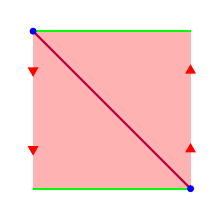
\begin{tikzpicture}

        % Define center points
        \node (top_orig) at (0,0) {};

        % draw the squares
        \draw[fill = red!30, draw = red!30] ($(top_orig) + (-1,-1)$) rectangle ($(top_orig) + (1,1)$);
        \draw[green, thick] ($(top_orig) + (-1,-1)$) -- ($(top_orig) + (1,-1)$);
        \draw[green, thick] ($(top_orig) + (-1,1)$) -- ($(top_orig) + (1,1)$);
        %\draw[dashed, red, thick] ($(top_orig) + (-1,-1)$) -- ($(top_orig) + (-1,1)$);
        %\draw[dashed, red, thick] ($(top_orig) + (1,-1)$) -- ($(top_orig) + (1,1)$);
        \draw[purple, thick] ($(top_orig) + (-1,1)$) -- ($(top_orig) + (1,-1)$);

        % draw the arrows
        \node[fill = red, regular polygon, regular polygon sides=3, shape border rotate=180, inner sep = 0.8] (arrow) at ($(top_orig) + (-1,0.5)$) {}; 
        \node[fill = red, regular polygon, regular polygon sides=3, shape border rotate=180, inner sep = 0.8] (arrow) at ($(top_orig) + (-1,-0.5)$) {}; 
        \node[fill = red, regular polygon, regular polygon sides=3, inner sep = 0.8] (arrow) at ($(top_orig) + (1,0.5)$) {}; 
        \node[fill = red, regular polygon, regular polygon sides=3, inner sep = 0.8] (arrow) at ($(top_orig) + (1,-0.5)$) {}; 

        % draw the corners
        \node[fill = blue, circle, inner sep = 0.9] (right_corner) at ($(top_orig) + (-1,1)$) {};
        \node[fill = blue, circle, inner sep = 0.9] (right_corner_2) at ($(top_orig) + (1,-1)$) {};

      \end{tikzpicture}
      \caption{The M\"obius strip as a cell complex.}
      \label{fig:Q3_Mobius_Cell}
\end{figure}

It is hopefully clear that this representation uses a single 2-cell, so $k = 1$.

\section*{Q4}
\subsection*{(a)}
Calculating the Euler characteristic of $T \times \mathbb{P}^2$ one has 

\begin{equation*}
    \chi(T \times \mathbb{P}^2) = \chi(T)\chi(\mathbb{P}^2) = \chi(S^1 \times S^1)\chi(\mathbb{P}^2) = \chi(S^1)\chi(S^1)\chi(\mathbb{P}^2) = 0
\end{equation*}

as $\chi(S^1) = 0$. Furthermore $\chi(S^4) = 2$ (in both cases, we use the results of exercise 5.22). 
Since the Euler characteristic is fixed under homeomorphism this shows that these spaces are not 
homeomorphic.

\subsection*{(b)}
Let $f:Y\rightarrow X$ be a continuous function from some topological 
space $Y$ to a contractible space $X$. Since $X$ is contractible there exists some deformation retraction $R:X\times[0,1]\rightarrow X$ such that $R(x,0) = 1_{X}$ 
and $R(x,1) = x_0$ for some $x_0 \in X$. Therefore one can define $F:X\times[0,1] \rightarrow Y$ 
as $F(x,t) = R(f(x),t)$ with $F(x,0) = f(x)$ and $F(x,1) = x_0$. This function is continuous as 
$f$ and $R$ are continuous, so $f \overset{F}{\sim} x_0$ where $x_0$ is the constant function. Since our choice of $f$ was arbitrary, for any two continuous functions 
$f,g:Y\rightarrow X$ it follows that $f \sim x_0 \sim g \implies f \sim g$. So both these 
functions are homotopic.

\paragraph{}
If $f:S^n\rightarrow S^n$ is not onto, then it can be expressed as $f:S^n \rightarrow S^n\backslash \{p\}$ 
for some $p \in S^n$. However $S^n\backslash \{p\}$ is homeomorphic to $E^n$, which is clearly 
contractible. From the proof above, this implies that $f$ is homotopic to a constant 
function. So for $f:S^n\rightarrow S^n$, it must be either onto or homotopic to a constant function.

\section*{Q5}
\subsection*{(a)}
Let $x^* \in W$ be a point in $W$ such that for all $y \in W$ 
the segment of the line that passes through both these points is in $W$ between both of these points. 
Then consider $R(x,t):W\times[0,1]\rightarrow W$, $R(x,t) = tx^* + (1-t)x$. For any 
particular direction in $x_i$ in $x = [x_1,x_2,x_3,\dots,x_n]$ one has 

\begin{equation*}
    R(x,t)_i = tx_i^* + (1-t)x_i
\end{equation*}

so for all $\epsilon > 0$ one can choose $\delta_i < \max\{(|x^*_i| + 2 + |x_i| + |t|)\epsilon,1\}$. Then for 
$x',t'$ such that $|x - x'| < \delta_i$, $|t-t'| < \delta_i$ one obtains

\begin{align*}
    |r(x,t) - r(x',t')| &\leq |x^*_i||t - t'| + |x_i-x_i'| + |tx_i - t'x_i'| \\
    &\leq \delta_i(|x^*_i| + 1) + |x_i(t-t')| + |t'(x_i-x_i')| \\
    &\leq \delta_i(|x_i^*| + 1 + |x_i| + |t'|) \\
    &\leq \delta_i(|x_i^*| + 1 + |x_i| + |t| + \delta_i) \\
    &\leq \delta_i(|x_i^*| + 2 + |x_i| + |t|) < \epsilon
\end{align*}

If we take $\delta = \min\{\delta_1,\delta_2,\dots,\delta_n\}$ then this function is 
continuous under the infinity norm and thus in Euclidean topology. Since $R(x,0)$ is the 
identity map and $R(x,1) = x^*$ for all $x \in W$, $R$ is a deformation retract and so 
$W$ is contractible.

\subsection*{(b)}
See \autoref{fig:Q5_cone} for a sketch of $S$ (note that $S$ continues indefinitely in the $z$ direction). 

\begin{figure}[H]
    \centering
    
    \begin{tikzpicture}[tdplot_main_coords]
        \coordinate (O) at (0,0,0);
        \draw[-] (0,0,-2) -- (0,0,-1) {};
        \coneback[surface=black]{-1}{1}{-10}
        \conefront[surface = white]{-1}{1}{-10}
        \draw[->] (-6,0,0) -- (6,0,0) node[right] {$x$};
        \draw[->] (0,-6,0) -- (0,6,0) node[right] {$y$};
        \coneback[surface=black]{3}{3}{10}
        \conefront[surface=white]{3}{3}{10}
        \draw[->] (0,0,3) -- (0,0,3.8) node[above] {$z$};
        
    \end{tikzpicture}
    \caption{A sketch of $S$.}
    \label{fig:Q5_cone}
\end{figure}

In cylindrical coordinates, this surface can be written as 

\begin{equation*}
    S = \{(r,\theta,z): \theta \in [0,2\pi),\, r \leq z, \, z \geq -1\}
\end{equation*}

It is hopefully obvious that for any particular point $(r^*,\theta^*,z^*) \in S$ the 
parametric line $l(t) = ((1-t)r^*,\theta^*,(1-t)z^*)$ lies inside $S$ for 
$t \in [0,1]$ and connects $(r^*,\theta^*,z^*)$ to the origin. Therefore by part (a) 
this space is contractible.

\end{document}
